Bitcoin is a technology that crossroads several disciplines:
\begin{itemize}
    \item cryptography
    \item game theory
    \item network and distributed systems
    \item monetary theory and economics.
\end{itemize}
It is not only a technology but also a paradigm shift with relevant legal, political and society implication.

\section{Internet e-cash}
The idea of an electronic cash system comes long before Bitcoin: a method whereby on the internet you can transfer funds from A to B without A knowing B or B knowing A.

David Chaum, the real cyberpunk movement's godfather, proposed \emph{e-cash} at the starting of the 80s, and it is based on \emph{blind signatures}.
It was implemented via his company, DigiCash, in 1990.

In this technology bank cannot trace money transfer only guarantees no double spending occurs.
Despite the initial interest and bringing large banks on board to use the system, e-cash never fully took off and DigiCash filed for bakruptcy in 1998.

\subsection{Blind signature}
In blind signature we have Alice that wants to send amount $x$ to Bob and there is a bank who can check for double spending, without knowing the amount.
\begin{itemize}
    \item Alice generates a random number called \emph{nonce} and mathematically combines it with a piece of data in order to appear like yet another random string of numbers;
    \item Alice then gives the scrambled data to the bank to sign and get bank a \emph{blind signature}.
    The blind signature is not only linked to Alice's keys and to the scrambled data but it is also linked to the original, unscrambled data;
    \item Using only bank's public key and the original data, anyone can check that the bank signed a scrambled version of the original data.
\end{itemize}

\section{Bitcoin}
In October 2008 an anonymous person (or a group) under the pseudonym Satoshi Nakamoto published the Bitcoin whitepaper and in January 2009 it released the code.
Satoshi then vanished in mid-2010 stopping any interaction.

Bitcoin is:
\begin{itemize}
    \item a purely p2p version of digital cash with no controlling authority, no servers and no bank as in e-cash;
    \item permissionless because there is no regulator;
    \item censorship resistant: so no frozen funds;
    \item free: so negligible transaction costs (not true anymore);
    \item borderless;
    \item transnational;
    \item cross-jurisdictional: no jurisdiction applies;
    \item default setting is suspicion in a completely untrusted environment;
    \item a solution for double spending, so Bitcoin can grow legitimately.
\end{itemize}

Moreover bitcoin offers pseudo anonimity because transactions doesn't disclose identity, it's like paying cash, addresses as pseudonyms but it's not possible to bind an address to a person unless the owner does it publicly.

Some motivations from the bitcoin movement are:
\begin{itemize}
    \item ideological reasons: cryptoanarchy and cyberpunk movement;
    \item good timing due to financial crisis in 2008: bitcoin was felt like a child of the crisis;
    \item bitcoin as digital gold: controlled supply enforced by the protocol and no intervention on money supply;
    \item bitcoin as an investment asset;
    \item presence of exchange, which are places where bitcoin are exchanged for mainstream fiat currencies;
    \item payments can be cheap;
    \item bitcoin regulated markets are arising;
    \item hundreds of other crypto and tokens born in the last years.
\end{itemize}

It is important to notice that Bitcoin is the protocol, the software and the community around them, while bitcoin is the unit of the currency: bitcoin are sent using the Bitcoin protocol.

\subsection{Decentralized identity management}
Since there is no centralized certification authority the identity is bound to a key-pair: to create a new identity you just create a new key-pair:
\begin{itemize}
    \item $sk$ is the private key;
    \item $pk$ is the public key which looks random and nobody needs to know who is the owner of the public key, but the key speaks for the user's identity.
    Sometimes instead of the public key itself it's hash is used $Hash(pk)$.
\end{itemize}
Of course only the owner of $sk$ can control the identity.

Then looking at a transaction, if it's signature $sig$ verifies $verify(pk, data, sig)$ then we can assume that $pk$ generated that transaction. 

Bitcoin uses ECDSA as a signature algorithm and the keys are generated over the $secp256k1$ curve.
It is important to notice that this cryptosystem is not quantum resistant, so if (once) the quantum computer become bigger and bigger this cryptosystem will be broken.

However nothing in Bitcoin is encrypted, keys are used only to prove ownership of tokens, transactions are public and messages on the blockchain too.

\subsection{Generation of bitcoing address}
To generate a Bitcoin address you:
\begin{itemize}
    \item generate a ECDSA private key;
    \item from the private key you obtain a 512 bit ECDSA public key with prefix;
    \item SHA256 of public key with prefix;
    \item RIPEM160 of SHA256 output;
    \item encode the RIPEM160 result and the checksum to base58.
\end{itemize}
The result of this process is the actual bitcoin address.

NB: Base58 is an encoding which uses all the alphanumeric alphabet removing all the easily mistakable characters (like 0, O, I, l).
This encoding can represent large numbers in a shorter format avoiding awkward characters.

\subsection{Workflow of Bitcoin Payment}
Let's suppose Alice wants to send tokens to Bob:
\begin{itemize}
    \item Alice asks Bob's Bitcoin address (out of band, so not using the Bitcoin protocol);
    \item Bob answers with it's actual address or with a new one, to increase anonymity;
    \item Alice generates a transaction $t$;
    \item Alice broadcasts $t$ on the p2p network;
    \item miners collect broadcasted transactions into a candidate block and attempt to mine the block (resolve the PoW);
    \item once the block has been solved it is broadcasted and after a while it will become part of the blockchain.
\end{itemize}
Of course merchants needs to wait for confirmations on $t$ before providing actual goods.

\subsubsection{Transaction in Bitcoin}
A transaction takes money from the source address and moves them to the destination address.
However a transaction must move all the tokens from the source so we have always at least two outputs:
\begin{itemize}
    \item the recipient address: which is the actual destination address we want to send the money to;
    \item the change address: usually the same source address which will get back the remaining tokens we don't want to move to the destination.
    It is also possible to specify another address, maybe a second Alice's address.
\end{itemize}
All the input must be consumed:
\begin{figure}[H]
    \centering
    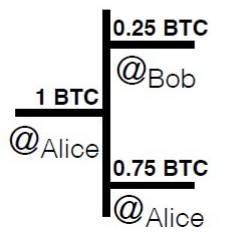
\includegraphics[width=70px]{images/6_Bitcoin/01.png}
    \caption{Transaction example}
\end{figure}

All the addresses we own are stored in a bitcoin wallet, which basically stores all the key-pairs.
Sometimes it's the Bitcoin client itself to generate a new address for the change address and store it in the wallet.

\subsubsection{Transaction fees}
Of course:
$$
    \sum inputs \geq \sum outputs
$$
if those values are not equal then we are setting up a \emph{fee} which is an optional amount which will be collected by those entities that will validate the transaction (miners).
It's a fair practice to shorten the validation time of the transaction because some miner can decide to mine only transactions with fees to increase their gain.

\subsubsection{Transaction forms}
Usually the transaction has one input and two outputs, however it's not mandatory, for example:
\begin{itemize}
    \item merging funds: aggregate several input into a single output.
    It's like exchanging a pile of coins or a single larger note.
    It's used to clean up a lots of smaller amounts that were received as change for payments.
    It's used for \emph{joint payments} along with multisignature transactions, because of course every input address must sign the transaction;

    \item distributing funds: one input and several outputs.
    It's a transaction which distributes the value in input to multiple recipients, it's used to distribute funds like processing payroll payments to multiple employee;

    \item multi input to multi output transactions: simply get funds from different inputs and distribute to different outputs.    
\end{itemize}

\subsection{UTXO model}
Centralized currencies use a balance number associated to the account (Ethereum too).
Bitcoin instead uses the Unspent Transaction Output (UTXO) model.

An \emph{unspent output address} is an address containing bitcoins which are not spent in any transaction yet.
Bitcoins are spread in several UTXO associated with the same address or with different addresses.
In every transaction each input is linked to a UTXO of a previous transaction and each transaction outuput generates a new UTXO which will then be included in the receiver's user wallet.
Of course once a UTXO is spent it is no longer a UTXO because we can't spend twice the same amount.

\begin{figure}[H]
    \centering
    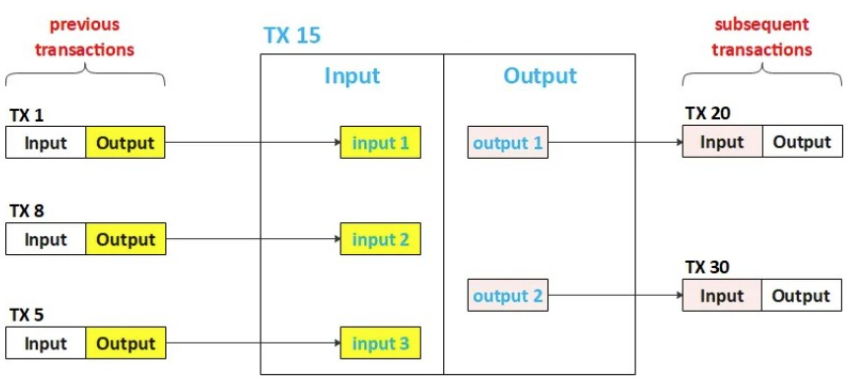
\includegraphics[width=300px]{images/6_Bitcoin/02.png}
    \caption{UTXO model}
\end{figure}

Each new UTXO locks the newly generated UTXO to the new owner's public key, once it wants to spend those bitcoins it can unlock the funds using it's private key.

This model allows to avoid storing the entire blockchain to prove a transaction, but only the effectively UTXO not yet spent, in fact in order to find the balance of an address we only need to add up all the UTXO locked to that address.

\subsection{Transaction scripts}
Each transaction contains some \emph{scripts} which are simple programs written in a simple programming language and are used mainly to verify the ownership of the transferred coins.
The language is not Turing complete in order to prevent infinite looping and error execution.

The language is based on a FORTH so it's a stack-based non-Turing complete language and is executable on a wide range of hardware.
Moreover it is:
\begin{itemize}
    \item stateless: no prior state to the execution script and no saved state after the execution of the script.
    The script is comprehensive of all the information needed, this is a key difference in respect to Ethereum.

    \item deterministic: a script will predictably execute the same way on any system, which is important in order to validate transactions;

    \item simple and compact: all the opcodes are 1 byte long, so there are 256 instructions:
    \begin{itemize}
        \item basic arithmetic: \verb|OP_ABS|, \verb|OP_ADD|, ...
        \item stack management: \verb|OP_DROP|, \verb|OP_SWAP|, ...
        \item flow control: \verb|OP_IF|, \verb|OP_ELSE|, (not while!)
        \item bitwise logic: \verb|OP_EQUAL|, \verb|OP_EQUALVERIFY|,
        \item crypto instructions for:
        \begin{itemize}
            \item hashing: \verb|OP_SHA1|, \verb|OP_SHA256|
            \item signature verification: \verb|OP_CHECKSIG|, \verb|OP_CHECKMULTISIG|,
            \item locktime: \verb|OP_CHECKLOCKTIMEVERIFY|
        \end{itemize}
    \end{itemize}
\end{itemize}

An example of usage of those scripts could be the usual bitcoin lock:
\begin{itemize}
    \item $A_1$ has some locked bitcoins and can unlock them;
    \item $A_1$ puts a small piece of code (a script) on top of the sent bitcoin that will lock the transferred bitcoin;
    \item when $A_2$ wants to spend its bitcoin it has to unlock them by providing another script;
    \item running the locking and the unlocking codes together will allow $A_2$ to spend the received bitcoin.
\end{itemize}
In this example the locking phase can be as simple as encrypting stuff with the public key of $A_2$ and the unlocking phase to decrypt with the $A_2$ private key, this way only $A_2$ can unlock the funds since he's the one who knows the private key.

More in general it's a piece of code that verifies a set of arbitrary conditions that must be met in order to spend coins.
Some other examples are:
\begin{itemize}
    \item simple signatures checks to redeem previous transaction signing it and put a signature that corresponds to the public key;
    \item Multi signature;
    \item pay-to-script-hash;
    \item proof-of-burn;
    \item escrow transactions;
    \item green addresses;
    \item micro payments.
\end{itemize}

\subsubsection{Pay to Pubkey (P2PK)}
It's the simplest script we can use and allows us to transfer some bitcoins to an address (namely a public key).
First things first we need to recall that:
\begin{itemize}
    \item the locking script is inside the output of the transaction;
    \item the unlocking script is inside the input of the transaction.
\end{itemize}
While spending something we concatenate both parts in a transaction, the VM executes them and we have our transaction.

The unlocking script of P2PK is \verb|OP_PUSH signature| while the locking script is \\
\verb|OP_PUSH PubKey, OP_CHECKSIG|, so once the VM concatenates those scripts we obtain the actual script to be executed to build the transaction.

It is important to notice that the signature is built by the owner of the bitcoins, so the one who wants to initiate the transaction and is the only one who knows the private key.

NB: the most common script is pay-to-public-key-hash (P2PKH) because we use the hash of the public key as the address, so we have:
\begin{itemize}
    \item unlocking script: \verb|OP_PUSH signature, OP_PUSH PubKey|;
    \item locking script: \verb|OP_DUP, OP_HASH160, OP_PUSH PubKeyHash,| \verb|OP_EQUALVERIFY, OP_CHECKSIG|.
\end{itemize}

\subsection{Structure of a real bitcoin transaction}
A real bitcoin transaction is an encoded JSON filled with some metadata:
\begin{verbatim}
    {
        "hash":         "...",
        "ver":          1,
        "vin_sz":       2,
        "vout_sz":      1,
        "lock_time":    0,
        "size":         404,
        ...
    }
\end{verbatim}
in which:
\begin{itemize}
    \item hash: is the hash of the entire transaction and is used as unique identifier;
    \item version: allows different interpretation of some fields, it is used to upgrade the protocol if some vulnerabilities are found;
    \item locktime: defines the earliest time that a transaction can be added to the blockchain:
    \begin{itemize}
        \item 0: execute the transaction immediately;
        \item otherwise: used in stuff like \emph{escrow} and for the lightning network.
    \end{itemize}
\end{itemize}

Of course among those metadata there are also the arrays for input transactions:
\begin{verbatim}
    "in": [
        {
            "prev_out": {
                "hash": "...",
                "n":    0
            },
            "scriptSig": "..."
        },
        ...
    ]
\end{verbatim}
in which:
\begin{itemize}
    \item the hash in \verb|prev_out| contains the hash of the input transaction;
    \item the \verb|n| contains the number of the output of the selected transaction;
    \item the \verb|scriptSig| contains the signature of the unlocking script we want to use
\end{itemize}

and the one for output:
\begin{verbatim}
    "out": [
        {
            "value": "10.122",
            "scriptPubKey": "OP_DUP OP_HASH160 69e...3d42
                OP_EQUALVERIFY OP_CHECKSIG"
        },
        ...
    ]
\end{verbatim}
in which:
\begin{itemize}
    \item \verb|value| is the amount we want to move;
    \item \verb|scriptPubKey| contains the locking script containing the receiving address 
\end{itemize}

\subsection{Transaction lifecycle}
Once the transaction has bee created, then it must be signed with one or more signatures indicating the authorization to spend the funds referenced by the transaction.
Then the transaction is broadcasted to the Bitcoin p2p network and each network node validates and propagates the transaction until it reaches every node in the network.
During the validation process each nodes checks:
\begin{itemize}
    \item if the previous outputs referenced by the transaction exist and have not been spent;
    \item the sum of the input values is greater or equal to the sum of the outputs;
    \item the signatures for the transaction input are valid so if each input is signed with the private key corresponding to the public key referenced in output script.
\end{itemize}
The transaction then needs to be verified by a mining node and included in a block of transactions recorded on the blockchain.

Once the block is recorded on the blockchain and confirmed by sufficient subsequent blocks (usually 6) the transaction is a permanent part of the blockchain and the fund transferred to the new user can be spent in a new transaction.

The algorithm when a new transaction is received is:
\begin{verbatim}
    receive transaction t
    for each input (h, i) in t:
        if output (h, i) is not in UTXO or signature invalid:
            drop t and stop

    if sum(inputs) < sum(output):
        drop t and stop

    for each input (h,i) in t:
        remove (h,i) from local UTXO

    append to to local memory pool (waiting for confirmation from miners)
    forward t to neighbors in the Bitcoin network
\end{verbatim}
This describes the \emph{local acceptance policy} but doesn't mean that the transaction accepted locally will be accepted globally too.
The unconfirmed transaction are added to a pool called \emph{local memory pool} and are added to the blockchain only once are globally confirmed.

\subsection{Nakamoto consensus}
In blockchain there is the needs of a procedure to reach a \emph{common agreement} in a distributed or decentralized multi-agent system.
In traditional distributed systems we demand reliability and fault tolerance which means we want correct operations in presence of faulty nodes (for example a node that suddenly crashes or becomes unavailable), a network partition or byzantine faults (a node starts behaving maliciously).
Aside from blockchains those algorithms are needed for example in database transactions when database is sharded, state machine replication and distributed clock synchronization.

Bitcoin uses \emph{nakamoto consensus} which is an implicit approach to consensus without voting or collective message passing algorithm executed by the nodes.
It builds \emph{eventual consistency} which means that occasionally nodes see an inconsistent view of the ledger (blockchain forks) but at some point everyone will see the same history of the ledger.
This works if majority of the nodes is honest, basically it works in practice but it's difficult to make theoretical proofs, because it's based on incentives from the network to collaborate and behave correctly.

\subsubsection{Why consensus is needed}
Let's suppose we don't use any consensus mechanism: once we receive a transaction we append it to the blockchain.
A user can issue two transactions with the same money and propagate them from two different nodes in the network.
Then those nodes will start to spread their ledgers until two adjacent nodes have the two different ledgers with the two different transactions.
None of those two nodes will take the other transaction since it would raise a double spending issues, we have two conflicting transactions and the network is splitted because there is no rule to agree on which of the two transactions is the valid one.

The network needs to reach consensus on which of the two values has to be added to the ledger before actively adding one of them.

\subsubsection{MemPool and competition}
Instead of adding transactions directly to the ledger we create a \emph{MemPool} which stores the transactions awaiting confirmation.
This way we can have conflicting transactions occuring in the MemPool and not in the ledger, so when the node receives a double spend which creates a conflicting transaction the node simply discards the received transaction.

Each node tries to get the transactions out from its MemPool and put them onto the ledger building a competition to add them.
The competition is based upon a lottery which prevents both transactions to be added to the ledger.
This competition is called \emph{mining} and the winner adds the valid transactions from its MemPool to the ledger and then broadcasts the new part to the neighbors. 

In case a node receives a ledger update which contains a transaction that conflicts with a transaction in the mempool then the node kicks that transaction out from its memory pool and propagates the ledger update.

\subsubsection{Bitcoin mining}
Mining is the process of trying to add a new block to the blockchain and it's a network-wide competition.
The mining process starts by creating a \emph{candidate block} with:
\begin{itemize}
    \item an header containing:
    \begin{itemize}
        \item \verb|version| of the protocol tracking bug fixes and new features, but also soft and hard forks;
        
        \item \verb|time|: local clock timestamp used for tuning difficulty of proof-of-work (see later), assert block creation and because there is no clock syncronization among nodes;
        
        \item \verb|mhash|: root of the Merkle tree of the transactions in the block.
        It is built on demand, so the block only stores the root hash;

        \item \verb|hashprev|: SHA256 hash of the previous block (top of the blockchain over which the miner builds the current block);

        \item \verb|target|: used in PoW;

        \item \verb|nonce|: used in PoW;
    \end{itemize}

    \item a transactions list with transactions taken from the memory pool (usually the one with the bigger fee in order to maximize the win in case of lottery win).
\end{itemize}
Any change to a transaction in the block results in a change the mhash and so the hash o the whole block.

\begin{figure}[H]
    \centering
    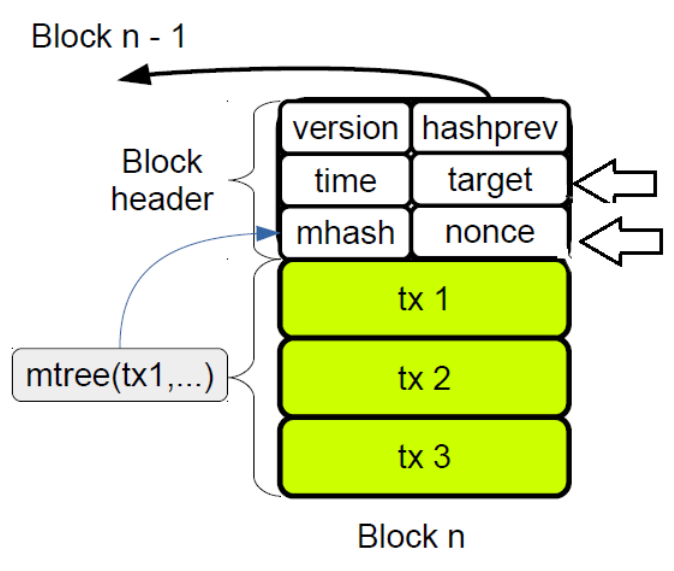
\includegraphics[width=200px]{images/6_Bitcoin/03.png}
    \caption{Block structure}
\end{figure}

The mining works like this:
\begin{itemize}
    \item set the value of the nonce of the block header to 0;
    \item hash the whole block header, including the nonce;
    \item check if the resulting hash is under the target.
    If the hash of the block header is not below the target just increment the nonce.
    This way we have always the same information in the block header but we get a completely different hash.
\end{itemize}
So basically the target defines the required number of zeros at the beginning of the PoW hash and the nonce is a 32 bit value that can be changed to find PoW via brute-force search.
Once we've found a hash that solves the PoW we've won the lottery.

Of course different blocks may have different target values, this is done in order to tune difficulty of PoW as the network size grows.

The key idea is to select a random node at each round, this selection is made proportionally to a resource that is hard to monopolize, in the case of Bitcoin this resource is computational power, and the selection is done on the basis of the Proof of work.

Of course once the PoW is solved we finish to build the block and spread it over the network, this way other nodes can check our PoW too and end the confirmation of our node by attaching the node to their ledger.

\subsubsection{Formal definition of PoW}
Let be:
\begin{itemize}
    \item $d$: the difficulty, a positive number which is used to adjust the time to execute the proof;
    \item $c$: challenge, a given string;
    \item $x$: nonce, an unknown string.
\end{itemize}
then the proof-of-work is a function:
$$
    F_d(c,x) \xrightarrow{} \{true, false\}
$$
satisfying the following properties:
\begin{itemize}
    \item $d$ and $c$ are fixed;
    \item $F_d(c,x)$ is fast to compute if $d$, $c$ and $x$ are known (the proof of PoW);
    \item instead finding $x$ so that $F_d(c,x) = true$ is computationally difficult, but feasible (the actual workload).
\end{itemize}

\subsubsection{Incentives}
Another incentive to the miner to continue to mine and to behave honestly is the block reward.
It's a payment to the miner in exchange for the service of creating a block.
The protocol itself \emph{mints} new coins when a new block is mined and it's the only way to create new bitcoins, aside from transaction fees we've discussed before.

The amount of bitcoins produced by each block halves every 4 years (every 210'000 blocks) until no more bitcoins will be produced, so there is a maximum amount of coins that the network will always have.

\begin{figure}[H]
    \centering
    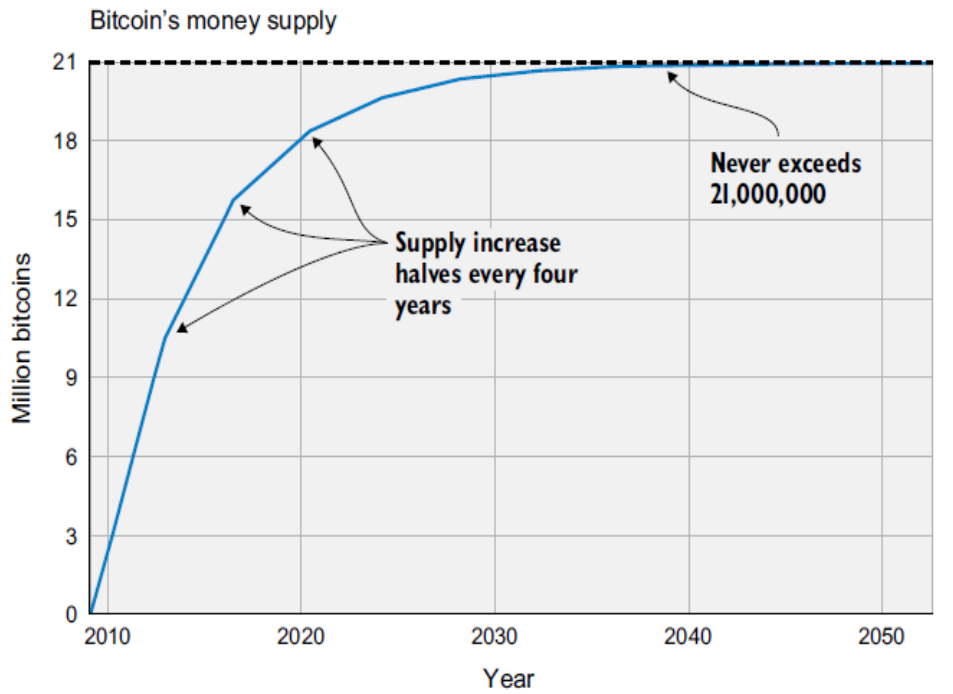
\includegraphics[width=250px]{images/6_Bitcoin/04.png}
    \caption{Bitcoin production}
\end{figure}


A \emph{coinbase} transaction is the first transaction in each block and encodes the transfer of reward and transaction fees to the miner, it does not consume previous unspent outputs contained in the blockchain and creates bitcoins from nothing.
The output address instead is the miner's one (or the various addresses of the miners involved).

\subsubsection{Longest chain rule}
In the simplest scenario no blocks are mined at the same time, in this case the propagation is simple and all the network will start to mine on top of that new block.

However there could be scenarios in which more than one block is mined almost at the same time, so a part of the network will receive the block $A$ and another part will receive the block $B$.
In this case we say that the blockchain gets forked.
Since it is very unlikely that the two forks will continue growing at the same ratio eventually one of them will become longer than the other chain and so the nodes will switch, reaching consensus at some point, making the other chain a dead branch.

This behavior may require a chain reorganization in whiche we move out blocks from an old active chain and put those transaction in the MemPool.
Of course miners of the blockchain are incentivized to build on the longest chain because it has a higher probability to be accepted, otherwise they will waste computational effort.

\section{Attacks}
Attacks on blockchain can come from different layers:
\begin{itemize}
    \item the p2p architecture
    \item the consensus mechanism
    \item the transactions.
\end{itemize}

\subsection{Double spending attack}
In this attack we try to spend the same bitcoin twice.

We can try to double spend the bitcoins by sending two transaction to the network.
In this case both transaction will go in the MemPool of the miners, only one will be inserted in the next block from an honest miner while the second one will be considered invalid, so not confirmed and discarded.

If instead the two transactions gets validated simultaneously by two different miners the blockchain forks, of course eventually one of them will be drop because of the longest chain rule.

Again if the miner is malicious, it can add both transactions in the same block and mine it.
Then once the miner sends the block to the network, the other miners will discard it because of its invalidity.

In every case the attack does not succeed!

In order for this attack to succeed the evil miner can: spend it's bitcoins on the real chain and start to reverse the longest chain.
By reversing the longest chain we mean mining in stealth mode (so without broadcasting the blocks) by removing it's transaction in it's version of the blockchain.
The attacker then waits for the goods or the service to reach him and then, publish it's stealthy blockchain.
This way we have a parallel blockchain in which the coins are not spent but the goods has been received by the attacker.
In order to let this attack succeed the attacker needs 51\% of the hashing power of the network in order to add blocks to his version of the blockchain faster and eventually build a longer chain.

\subsubsection{Mining pools}
Mining pool is a consortium of miner which publish their computational power and then share the rewards.
In 2014 Ghash.io came close to reaching 50\% but nothing happen because it was more lucrative to keep mining blocks and collecting block rewards than reversing a single transactions.


\subsection{Transaction malleability attack}
This attack is based on modifying a transaction hash (TXID) without modifying the signature of the transaction.
Recall that the transaction input are signed with the private key of the owner of the funds, which are then verified by each node who receives the transaction.
However the transaction id (TXID, transaction hash) is the SHA-256 of all the fields of the transaction data, so a node can change the unlocking script in such a way that:
\begin{itemize}
    \item the transaction has the same effect;
    \item the signature is still valid;
    \item the TXID changes
\end{itemize}
(by adding some useless instructions like \verb|OP_NOP| or \verb|OP_DUP, OP_DROP|).

With this attack an attacker can intercept a normal transaction and distribute the modified version through the network, now which transaction is the right one?

An attack scenario is the following:
\begin{itemize}
    \item Alice issues a payment to Bob and signs the transaction $TXID_{1}$;
    \item Bob alters Alice's transaction signature before $TXID_{1}$ is confirmed, resulting in a new transaction $TXID_{2}$;
    \item $TXID_{2}$ gets confirmed on the blockchain before $TXID_{1}$;
    \item Alice does not see her transaction confirmed
    \item Bob asks Alice for a new payment since the first one did not succeed;
    \item Bob receives twice the intended amount.
\end{itemize}
Alice gets scammed by Bob.

\subsubsection{Segregated witness}
It's a change of the structure of bitcoin transaction data to avoid a malleability attack.
The main idea is to separate all the malleable information into a separate \emph{witness data}, compute the TXID withut the unlocking script, so that the identifier will never be able to change.

\subsection{Denial of service}
It can happen when a miner decides to not include victim's transactions.
Of course if transactions from the victim never gets inserted in the next blocks the transaction never happens.
Here too since the network is so wide someone at some point will add this transaction to some block, unless more than 51\% of the network will decide to not.

\section{Mining and mining pool}
\subsection{Generations of mining}
During the years the mining difficulty increased so much and in order to be competitive, miners developer and used more technology to improve mining hash rate.
During the first generation miners used CPUs to mine blocks with a sequential search of the right nonce, someone exploited core parallelization on the few cores of the processor.
However SHA256 was computed in software because no specialized hardware was inside the CPUs.

The second generation exploited GPUs because they are designed for high-performance graphics and offer high parallelism which allows to compute different hashes in parallel with different nonces, with an increase in the throughput and also the possibility of overclocking.
This behavior brought upset in the normal GPU market (gaming) because the prices of the GPUs sky-rocketed, however a lot of gamers become miners.
This technique is a lot more powerful than CPU mining but however is an underuse of the GPU functionalities and consumes a lot of power, still with a low payout.

With FPGA (Field Programmable Gate Array) become the third generation.
Those devices can be programmed in Verilog which is a hardware design language and performance are as close as possible to the custom hardware, also they can be re-configured in case of protocol changes or blockchain switch.
It offers of course higher performance than GPUs, better cooling but are far more expensive than GPUs and marginal performance/cost advance over GPUs.

In the end ASIC (Application Specific Integrated Circuits) brought us the last generation so far.
They are special purpose hardware, so chip designed and built only for Bitcoin mining, so really fast to compute SHA-256.
They are also designed and produced very quickly but a lot expensive.

\subsection{Solo mining}
Solo mining is a Poisson process because it is a very risky task even if the reward is high.
Poisson process means that it has a large standard deviation, in fact it has a large incertitudes.

\subsection{Mining pools}
A pool is a group of small/large miners working together and sharing rewards.

\subsubsection{Centralized mining pools}
In centralized mining pools the pool manager coordinates a set of workers.
It sends block to all the miners and distributes revenues to the members based on the work they have performed, also taking a cut for itself (as a fee).
In this scenario the pool manager must be trusted by everyone.

The basic idea is that:
\begin{itemize}
    \item the mining pool operator sends to each worker a block-header containing data of some transactions including a coinbase transaction referring the reward to a private key owned by the operator itself;
    \item the miner then tries to fine the correct nonce to solve the block;
    \item if the miner finds the nonce then he sends it to the operator;
    \item once the nonce is found by some of the pool members each of them is rewarded proportionally to his work.
\end{itemize}

In order to understand if a node is doing the work it is actually claiming, and to measure the effort of each worker, in order to share fairly the single workers send to the mining controller the produced \emph{shares}.
A share is a \emph{near-valid block} or \emph{near optimal hash}, which is basically a hash that contains fewer zeros than those required by the current difficulty.
They are still rare to find so they are a good PoW to prove that a node is working as it claims.

There are various way to pay miners out:
\begin{itemize}
    \item pay per share: each miner gets instantly rewarded at the moment it presents a share.
    This guarantees a reward without waiting for the pool to find a block and doesn't allow any bonus to the miner who actually mines the block.
    Moreover this way risk is at the pool operator's who pays miners from pool's existing balance.
    It is important to notice that this way disadvantage workers to send valid blocks to the manager because they can discard valid blocks but still be paid the same reward.

    \item pay proportional: this way the amount of payment depends on whether or not the miner actually found a valid block.
    Every time a valid block is found, the rewards from that block are distributed to the members proportionally to how much work they actually did.
    Moreover the risk for the pool manager is lower because it pays only when valid blocks are found, this also incentivizes workers to send in the valid blocks that they find.    
\end{itemize}

In general if the pool is large enough the variance of how often the pool finds blocks will be fairly low.

\subsubsection{Decentralized mining pools}
It was adopted in 2011 by P2Pool and now used by other pool too.
In this solution a group of miners creates in parallel to Bitcoin a new network to build a separate and private chain which includes weak blocks mined with lower difficult until a valid block is found, then of course distribute reward through a this side blockchain, then merged to the main chain with \emph{merge mining}.

This mining pool is far more transparent and offers a fair payout scheme, moreover the performance overhead is minimal.
The idea is to create a parallel blockchain in which every node in this side blockchain adds their weak blocks until a valid block is found.
Each new node of this side chain contains addresses of each miner which added a block from the last valid block up to now, this can be used in order to track who actually worked, this list grows proportionally to the work done and once a valid block is found, it is already a coinbase block for all the miners who put power in that new block.

This approach avoids cheating because a node can't assert of having done work if it produced no blocks in the side chain, moreover this parallel chain can be audited to verify users effort.

\begin{figure}[H]
    \centering
    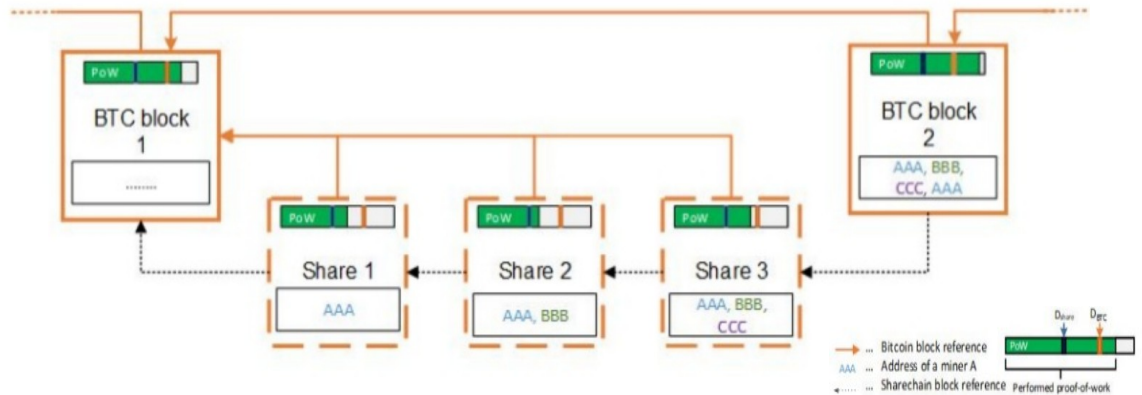
\includegraphics[width=330px]{images/6_Bitcoin/05.png}
    \caption{Side chain visualization}
\end{figure}





